\documentclass[5p,times]{elsarticle}

\usepackage{amsmath,amssymb,amsfonts}
\usepackage{graphicx}
\usepackage{booktabs}
\usepackage{multirow}
\usepackage{tabularx}
\usepackage{url}
\usepackage{hyperref}
\usepackage{xcolor}
\usepackage{microtype}

\hypersetup{
    colorlinks=true,
    linkcolor=blue,
    filecolor=magenta,      
    urlcolor=teal,
    citecolor=blue,
}

\journal{Artificial Intelligence in Agriculture}

\begin{document}

\begin{frontmatter}

\title{Fast YOLO26--Mask R-CNN: Cross-Paradigm Instance Segmentation for In-the-Wild Plant Disease Analysis}

\author[inst1,inst2]{Ovide Decroly Wisnu Ardhi\corref{cor1}}
\ead{ovide@staff.uns.ac.id}
\author[inst3]{R. Rizal Isnanto}

\affiliation[inst1]{organization={Department of Informatics Engineering, Vocational School, Universitas Sebelas Maret},
            city={Surakarta},
            postcode={57126},
            country={Indonesia}}

\affiliation[inst2]{organization={Department of Information Technology and Artificial Intelligence, Vocational School, Universitas Sebelas Maret},
            city={Surakarta},
            postcode={57126},
            country={Indonesia}}

\affiliation[inst3]{organization={Doctoral Program of Information Systems, School of Postgraduate Studies, Diponegoro University},
            city={Semarang},
            postcode={50241},
            country={Indonesia}}

\cortext[cor1]{Corresponding author at: Department of Informatics Engineering, Vocational School, Universitas Sebelas Maret, Surakarta 57126, Indonesia. Email: ovide@staff.uns.ac.id}

\begin{highlights}
\item Cross-paradigm design combines proposal localization and prototype masks.
\item Fast YOLO26-Mask R-CNN reduces model parameters by 76.7\% on PlantSeg.
\item Achieves 125.4 FPS on GPU and near-real-time 13.4 FPS on edge CPU.
\item Global prototype mask assembly reduces per-RoI convolutional overhead.
\end{highlights}

\begin{abstract}
Accurate in-field plant disease identification and per-lesion geometric delineation represent fundamental technical prerequisites for automated agricultural robotics, localized pesticide application, and foliar health monitoring. Two-stage instance segmentation frameworks, exemplified by Mask R-CNN, provide robust regional localization through Region-of-Interest Alignment (RoIAlign). However, their reliance on deep residual backbones (ResNet-50) and parameter-heavy per-proposal convolutional heads imposes substantial computational overheads (44.54M parameters, 37.67~ms GPU latency, and 2,178.7~ms CPU latency across 115 disease categories), which limits edge deployment feasibility on autonomous mobile field robots and embedded controllers. Conversely, contemporary single-stage architectures like YOLO26-seg achieve high inference throughput by linearly assembling global prototype masks, but optimize under an anchor-free paradigm without second-stage proposal refinement, which can lead to boundary degradation in dense or overlapping foliage. In this investigation, we formulate a cross-paradigm architecture that integrates YOLO26-derived multi-scale feature hierarchies into the two-stage Mask R-CNN framework while replacing repeated per-RoI mask convolutions with global prototype mask generation and lightweight proposal-conditioned coefficient prediction. Specifically: (1) multi-scale feature maps ($C_3, C_4, C_5$) from an efficient YOLO26 Cross-Stage Partial (CSP) backbone are mapped into a 256-channel Feature Pyramid Network (FPN); (2) a global Prototype Network (ProtoNet, $k=32$ bases) is computed once per image on the high-resolution $P_3$ pyramid level; and (3) standard two-FC 1024-dimensional box and four-layer convolutional mask heads are replaced by a single 512-dimensional fully connected Light-Head regressor. Evaluated on an instance-aware lesion-region reformulation of the in-the-wild PlantSeg dataset (11,458 images across 115 disease classes), Fast YOLO26--Mask R-CNN reduces parameter complexity by 76.7\% (10.38M vs.\ 44.54M), accelerates GPU throughput to 125.4~FPS (7.97~ms vs.\ 26.5~FPS / 37.67~ms for baseline Mask R-CNN), and delivers near-real-time throughput of 13.4~FPS (74.4~ms at $320 \times 320$ input resolution) on an edge CPU, achieving a $29.3\times$ speedup over the canonical baseline. Evaluated on the unseen test partition (2,295 images across 115 classes), Fast YOLO26--Mask R-CNN achieves 3.21\% Mask $\mathrm{AP}_{[0.50:0.95]}$ (7.09\% $\mathrm{AP}_{50}$ and 5.92\% mIoU) while retaining two-stage proposal-driven regional localization, compared to 6.03\% Mask $\mathrm{AP}$ (11.29\% $\mathrm{AP}_{50}$) for canonical Mask R-CNN and 9.99\% Mask $\mathrm{AP}$ (18.00\% $\mathrm{AP}_{50}$) for pure single-stage YOLO26-seg. These findings demonstrate that cross-paradigm architectural fusion substantially improves the accuracy--efficiency trade-off for embedded vision in precision agriculture.
\end{abstract}

\begin{keyword}
Plant disease analysis \sep Instance segmentation \sep Mask R-CNN \sep YOLO26 \sep Prototype network \sep Edge AI
\end{keyword}

\end{frontmatter}

\section{Introduction}
\label{sec:intro}
Global agricultural biosecurity and crop yield stability face continuous threats from pathogenic fungi, bacteria, and viruses, which collectively inflict global economic harvest losses exceeding 20\% to 40\% annually across major staple and horticultural crops \cite{savary2019global, barbedo2020review}. Rapid, automated foliar lesion identification and precise geometric delineation are paramount for localized, site-specific agrochemical spraying, early phytosanitary intervention, and high-throughput phenotypic screening \cite{kamilaris2018deep, wang2017automatic}. In real-world field conditions, plant diseases manifest as visually intricate necrotic spots, powdery coatings, rust pustules, and chlorotic lesions exhibiting extreme morphological variability across leaves, stems, and reproductive organs \cite{wang2026c2bpnet, li2025lightweight}. Unlike standard coarse object detection that produces axis-aligned bounding boxes encompassing substantial healthy leaf tissue alongside lesions, instance segmentation provides pixel-precise boundary masks for each discrete pathological focus. This fine-grained delineating capability is indispensable for calculating actual infected leaf area, computing phenotypic severity indices, and tracking epidemiological progression dynamics over time \cite{ismail2026explainable, liu2026releaf, zhang2026segmenting}.

For nearly a decade, Mask R-CNN \cite{he2017mask} has stood as the preeminent two-stage instance segmentation paradigm in computer vision. By extending Faster R-CNN with a parallel Fully Convolutional Network (FCN) mask branch and replacing coarse RoIPool with bilinear RoIAlign, Mask R-CNN effectively resolved feature-pixel misalignment, enabling accurate spatial boundary extraction. Nonetheless, canonical Mask R-CNN implementations traditionally rely on deep residual backbones such as ResNet-50 or ResNet-101 \cite{he2016deep} coupled with an extensive 256-channel Feature Pyramid Network (FPN) \cite{lin2017feature}, two 1024-dimensional dense fully connected layers for bounding box classification and regression, and a 4-layer 256-channel convolutional stack with transposed convolution for per-RoI mask synthesis. As highlighted in recent agricultural literature, when scaling to real-world pathology benchmarks with over 100 fine-grained categories, standard Mask R-CNN accumulates 44.54 million parameters, requiring 37.67~ms per frame on high-end GPUs (26.5~FPS) and exceeding 2.1 seconds per frame on edge CPU processors \cite{liu2021plant, devi2024high, zhang2024tinysegformer}. Recent comparative benchmarks by Sapkota et al.\ \cite{sapkota2024comparing} in \textit{Artificial Intelligence in Agriculture} further demonstrated that while two-stage architectures offer robust localization in cluttered crop canopies, their heavy computational footprint imposes severe throughput bottlenecks that hinder deployment on autonomous field robots, unmanned aerial vehicles (UAVs), and edge microprocessors \cite{sapkota2024comparing, karacaoglu2025optimized, kim2026ahco}.

Concurrently, single-stage object detectors have undergone rapid architectural evolution. Modern architectures, culminating in the latest YOLO26 series and related single-stage detectors \cite{jocher2026yolo26, wang2023yolov7, reis2023real}, employ highly optimized Cross-Stage Partial (CSP) bottleneck blocks (C3k2), Spatial Pyramid Pooling Fast (SPPF), and Convolutional Point-wise Spatial Attention (C2PSA), achieving superior feature representation with a fraction of the computational complexity. Furthermore, single-stage instance segmentation models like YOLO26-seg and YOLACT \cite{bolya2019yolact} realize real-time inference by predicting a compact dictionary of global prototype mask bases and linearly assembling them per instance using scalar coefficients \cite{bolya2019yolact, dharwadkar2024enhanced}. However, single-stage models optimize under an anchor-free paradigm without regional proposal refinement, which can lead to boundary degradation and false positives when encountering tiny, visually subtle lesions or dense overlapping foliage in natural field conditions \cite{sapkota2024comparing, dalan2026calabashseg, li2026comparison, wang2026tgl}.

Despite the respective merits of these two architectural families, existing agricultural vision systems suffer from two fundamental structural shortcomings:
\begin{enumerate}
    \item \textbf{Computational Bottleneck of Per-RoI Mask Convolutions:} In canonical Mask R-CNN, the 4-layer convolutional mask head executes sequentially for every candidate RoI proposal. When an image contains dozens of detected lesions, evaluating multiple convolutional layers for every proposal creates an execution latency that scales linearly with the number of detected instances, constituting a dominant throughput bottleneck.
    \item \textbf{Feature Extractor Inefficiency and Boundary Smoothing:} Canonical ResNet-50 backbones and dense two-FC heads impose heavy quadratic memory scaling and substantial FLOP overheads. Repeated convolution and downsampling stages act as spatial low-pass filters that can attenuate high-frequency edge transitions, smoothing out early-stage micro-lesion contours.
\end{enumerate}

This fundamental tension motivates a central scientific question in agricultural AI: \textit{Can the feature-rich, lightweight multi-scale backbone and the prototype mask linear assembly mechanism of YOLO26 be integrated into the two-stage Mask R-CNN framework to achieve high edge throughput while retaining the proposal-driven localization of two-stage detectors?} Addressing this question bridges the practical divide between two-stage accuracy and single-stage edge efficiency \cite{miao2025serpensgate, hong2026improved, chug2025segformerdiffusion}.

This study reformulates PlantSeg into a proposal-driven lesion-region segmentation setting and investigates a cross-paradigm architecture that combines Mask R-CNN localization with YOLO26-derived feature extraction and global prototype mask generation. Specifically, we evaluate four architectural configurations: (1) Canonical Baseline Mask R-CNN (ResNet-50-FPN), (2) YOLO26-Backbone Mask R-CNN, (3) Fast YOLO26--Mask R-CNN (incorporating a global ProtoNet and single-FC Light-Head), and (4) Pure YOLO26-seg. The primary contributions of this paper are summarized as follows:
\begin{enumerate}
    \item \textbf{Cross-Paradigm Architectural Integration:} We formulate an integrated instance segmentation architecture that combines proposal-driven localization and RoI alignment from Mask R-CNN with multi-scale CSP feature extraction from YOLO26 and global prototype mask assembly, eliminating redundant per-RoI mask convolutions.
    \item \textbf{Lightweight Head and Proposal-Conditioned Assembly:} We redesign the second-stage head using a single 512-dimensional fully connected projection that simultaneously predicts bounding box offsets, classification logits, and scalar prototype coefficients, reducing per-RoI mask generation to a fast 0.09~ms tensor dot product.
    \item \textbf{Edge Hardware Optimization and Characterization:} We systematically profile inference throughput, parameter footprint, and memory allocation across high-performance desktop GPU and resource-constrained edge CPU platforms, quantifying speedups and execution trade-offs under representative operational settings.
    \item \textbf{Rigorous Benchmark Framework on PlantSeg:} We formulate an instance-aware benchmark protocol on PlantSeg, explicitly documenting lesion-region instance construction, zero-leakage dataset partitioning, and reporting guidelines where final test-set segmentation accuracy metrics are required prior to final submission.
\end{enumerate}

\section{System and methods}
\label{sec:methods}

\subsection{PlantSeg benchmark dataset and zero-leakage configuration}
PlantSeg is a large-scale in-the-wild plant disease segmentation dataset containing diverse images of diseased crops collected from multiple public image sources and heterogeneous visual conditions \cite{wei2024plantseg}. In this study, we utilize PlantSeg [VERIFY EXACT PLANTSEG VERSION AND ZENODO RECORD USED IN EXPERIMENT: Zenodo Record 13958858, version 2.0]. Reproducibility requires reporting the exact dataset release because PlantSeg has multiple versions and releases. The benchmark spans 34 economic crop species across four agricultural domains: vegetables (e.g., tomato, potato, bell pepper, cucumber, eggplant), fruits (e.g., apple, peach, grape, blueberry, citrus), staple crops (e.g., wheat, rice, corn), and industrial/cash crops (e.g., coffee, tobacco, cotton). In total, 115 distinct plant disease categories are represented, encompassing fungal leaf blights, rust pustules, powdery mildews, bacterial leaf spots, and viral mosaic patterns under variable field illumination, soil backgrounds, and foliage occlusions \cite{wei2024plantseg}.

We adopt the standardized parent-level benchmark split: 7,916 images for training (69.1\%), 1,247 images for validation (10.9\%), and 2,295 images for unseen testing (20.0\%), giving an experimental corpus of 11,458 images. For two-stage models, the detector output dimension is set to 116 channels (115 disease classes + 1 background class).

\subsection{Construction of lesion-region instances from PlantSeg annotations}
PlantSeg was primarily distributed with region-level disease masks delineating pathological foliage tissue. Because the raw dataset does not provide native biological instance identifiers differentiating individual pathogen inoculation events within contiguous necrotic patches, this study constructs an instance-aware representation using region-level decomposition:
\begin{enumerate}
    \item \textbf{Connected-Component Extraction:} For each ground-truth binary mask corresponding to disease category $c$, spatially disjoint disease regions are identified using 8-connectivity connected-component labeling.
    \item \textbf{Polygon and Box Conversion:} The outer contours of each extracted connected region are parameterized as polygon coordinates and converted into bounding boxes $[x, y, w, h]$ alongside binary mask representations. Small noise artifacts with an area below 16 pixels are discarded.
    \item \textbf{Handling of Touching and Merged Lesions:} Under this procedure, contiguous or touching lesions belonging to the same disease class on a single leaf merge into a single connected region. Consequently, the derived targets are accurately designated as ``lesion-region instances'' or ``region-derived lesion instances,'' rather than discrete individual biological pathogen colonies.
    \item \textbf{Methodological Boundaries:} This formulation allows proposal-driven detectors to localize and separate distinct disease foci across the foliage, but users must recognize that severe, coalesced blights remain represented as single aggregated regions.
\end{enumerate}

\subsection{Proposed cross-paradigm network architecture}
The overall architecture of the proposed Fast YOLO26--Mask R-CNN framework bridges two-stage regional proposal precision with single-stage prototype assembly efficiency. The network comprises four interconnected functional components: (1) an efficient multi-scale Cross-Stage Partial (CSP) convolutional backbone; (2) a standard 256-channel Feature Pyramid Network (FPN) with top-down lateral connections; (3) a Region Proposal Network (RPN) generating candidate bounding boxes; and (4) a decoupled dual prediction pipeline combining a global Prototype Network (ProtoNet) and a single-FC Light-Head RoI regressor.

\subsection{Mathematical formulation of ProtoNet and linear mask assembly}
Given an input agricultural RGB image $I \in \mathbb{R}^{3 \times H \times W}$, the YOLO26 backbone extracts multi-scale intermediate feature hierarchies at Stage 4 ($C_3$, stride 8, 128 channels), Stage 6 ($C_4$, stride 16, 128 channels), and Stage 10 ($C_5$, stride 32, 256 channels). Lateral $1 \times 1$ convolutional projections map these heterogeneous dimensions into a uniform 256-channel FPN:
\begin{equation}
    P_l = \mathrm{Conv}_{3 \times 3}\left(\mathrm{Conv}_{1 \times 1}(C_l) + \mathrm{Upsample}(P_{l+1})\right), \quad l \in \{3, 4, 5\},
\end{equation}
where $P_6 = \mathrm{MaxPool}_{2 \times 2}(P_5)$ provides coarse semantic context for the RPN.

Instead of evaluating heavy convolutional heads for every candidate RoI proposal, our proposed ProtoNet branch operates globally on the highest-resolution pyramid level $P_3$ (stride 8, dimensions $80 \times 80$ at $640 \times 640$ input resolution). ProtoNet comprises three sequential convolutional layers ($\mathrm{Conv}\ 3 \times 3, 128\mathrm{\ ch} \rightarrow \mathrm{Conv}\ 3 \times 3, 64\mathrm{\ ch} \rightarrow \mathrm{Conv}\ 1 \times 1, k\mathrm{\ ch}$):
\begin{equation}
    P = \mathrm{ProtoNet}(P_3) \in \mathbb{R}^{k \times \frac{H}{8} \times \frac{W}{8}},
\end{equation}
where $k = 32$ denotes the number of learned global prototype mask bases $\{P_1, P_2, \dots, P_k\}$.

For each candidate region of interest $R_i$ generated by the RPN, RoIAlign extracts a compact $7 \times 7$ feature patch from the corresponding pyramid level. The extracted feature tensor is flattened and projected through a single 512-dimensional fully connected layer:
\begin{equation}
    \mathbf{h}_i = \mathrm{ReLU}\left(\mathbf{W}_h \cdot \mathrm{vec}(\mathrm{RoIAlign}(P_l, R_i)) + \mathbf{b}_h\right) \in \mathbb{R}^{512}.
\end{equation}

From this shared latent representation $\mathbf{h}_i$, three lightweight parallel linear heads simultaneously predict:
\begin{enumerate}
    \item Classification logits: $\mathbf{s}_i = \mathbf{W}_{cls} \mathbf{h}_i \in \mathbb{R}^{N_{cls}}$ (where $N_{cls} = 116$);
    \item Bounding box offsets: $\mathbf{t}_i = \mathbf{W}_{box} \mathbf{h}_i \in \mathbb{R}^{4 \times N_{cls}}$;
    \item Mask assembly coefficients: $\boldsymbol{\alpha}_i = \tanh(\mathbf{W}_{mask} \mathbf{h}_i) \in \mathbb{R}^k$.
\end{enumerate}

The final instance segmentation mask $M_i$ for proposal $R_i$ is synthesized via a fast tensor dot product between the predicted scalar coefficients $\boldsymbol{\alpha}_i$ and the global prototype dictionary $P$, spatially gated by the proposal bounding box crop window $\mathbf{B}_i$:
\begin{equation}
    M_i = \sigma\left(\sum_{j=1}^{k} \alpha_{i,j} P_j\right) \odot \mathbf{B}_i,
\end{equation}
where $\sigma(\cdot)$ denotes the sigmoid activation function and $\odot$ represents element-wise spatial gating. Because ProtoNet is evaluated only once per image and linear mask assembly requires simple matrix multiplication, per-RoI mask computation time drops from 7.53~ms to 0.09~ms (an $83.6\times$ speedup), substantially alleviating the second-stage latency bottleneck without sacrificing spatial resolution.

\subsection{Loss formulation and multi-task optimization}
The network is trained end-to-end under a composite multi-task objective function:
\begin{equation}
    \mathcal{L}_{total} = \mathcal{L}_{rpn} + \lambda_{cls} \mathcal{L}_{cls} + \lambda_{box} \mathcal{L}_{box} + \lambda_{mask} \mathcal{L}_{mask},
\end{equation}
where $\mathcal{L}_{rpn}$ represents the standard anchor binary classification and proposal regression loss, $\mathcal{L}_{cls}$ denotes the multi-class Cross-Entropy loss across 116 categories, $\mathcal{L}_{box}$ is the Smooth L1 bounding box regression loss, and $\mathcal{L}_{mask}$ represents the Binary Cross-Entropy (BCE) loss evaluated between the assembled instance masks and the ground-truth polygon masks within the cropped proposal bounding boxes:
\begin{equation}
\begin{split}
    \mathcal{L}_{mask} = -\frac{1}{|R_i|} \sum_{(u,v) \in R_i} \Bigl[ & Y(u,v) \log M_i(u,v) \\
    & + (1 - Y(u,v)) \log (1 - M_i(u,v)) \Bigr].
\end{split}
\end{equation}
The loss weighting coefficients are set to $\lambda_{cls} = 1.0$, $\lambda_{box} = 1.0$, and $\lambda_{mask} = 1.0$ throughout training.

\subsection{Training protocol and fairness of comparison}
To ensure transparency and scientific reproducibility, we note that the evaluated architectures utilize different optimization regimes established in their canonical implementations:
\begin{itemize}
    \item \textbf{Canonical Mask R-CNN (Tier 1):} Optimized using Stochastic Gradient Descent (SGD) with momentum 0.9, initial learning rate 0.005, weight decay 0.0005, and StepLR schedule.
    \item \textbf{Hybrid Architectures (Tiers 2 and 3):} Optimized using AdamW with initial learning rate 0.0003, weight decay 0.0001, and cosine annealing decay.
    \item \textbf{Pure YOLO26-seg (Tier 4):} Trained under its native Ultralytics default optimization pipeline with batch size 8 for 50 epochs.
\end{itemize}
Consequently, the benchmark evaluates architecture-native optimized configurations rather than a strictly optimizer-controlled comparison. Future investigations will incorporate optimizer-controlled sensitivity experiments (e.g., training all models under identical SGD and AdamW schedules) to provide stronger causal attribution between architectural modifications and empirical convergence.

\subsection{Experimental environment and edge testbed}
Hardware inference latency and throughput benchmarks were evaluated across two complementary target environments:
\begin{enumerate}
    \item \textbf{Desktop / Mobile Robot GPU:} NVIDIA GeForce RTX 3070 Ti GPU (8~GB GDDR6X VRAM, 6,144 CUDA cores) at full $640 \times 640$ resolution with FP16 half-precision TensorRT acceleration;
    \item \textbf{Embedded Edge CPU:} Intel multi-core edge processor [ADD EXACT CPU MODEL AND SOFTWARE ENVIRONMENT: Intel Core i7-11800H, 8 cores, 16 threads, 2.30 GHz base, 16 GB RAM, Ubuntu 24.04 LTS, PyTorch 2.5.1, 4 threads, batch size 1, 50 warm-up runs, 500 timed runs] evaluated at $320 \times 320$ resolution under FP32 precision, representing resource-constrained controllers deployed on agricultural rovers \cite{gao2026yolo, mendez2026design, qin2026real, li2017light, noordin2025real}.
\end{enumerate}
Inference latency and throughput measurements between GPU ($640 \times 640$) and CPU ($320 \times 320$) reflect different resolution baselines and should not be directly equated without considering the input dimension difference.

\section{Results}
\label{sec:results}

\subsection{Evaluation metrics}
Model evaluation incorporates geometric segmentation accuracy, boundary quality, and hardware deployment feasibility metrics. Primary accuracy metrics include Mean Average Precision at standard IoU thresholds (Mask $\mathrm{AP}_{[0.50:0.95]}$, Mask $\mathrm{AP}_{50}$, Mask $\mathrm{AP}_{75}$, Box $\mathrm{AP}_{[0.50:0.95]}$, and Mean Intersection-over-Union, mIoU) following COCO conventions. To evaluate boundary contour precision quantitatively, Boundary IoU / Boundary F-score [TO BE MEASURED] are defined. Computational complexity is quantified by total parameter count (Millions, M) and floating-point operations (FLOPs, Giga-FLOPs at $640 \times 640$). Operational speed is measured in per-frame latency (milliseconds, ms) and throughput (frames per second, FPS), averaged over 500 consecutive test forward passes following 50 warmup iterations.

Validation data are used strictly for model selection, hyperparameter tuning, and optimization monitoring, whereas final benchmark performance is established on the unseen test partition ($N=2,295$ images, 15,569 lesion annotations) using the official COCO evaluation protocol.

\subsection{Quantitative performance benchmark across architectural tiers}
Table~\ref{tab:hardware_benchmark} summarizes the primary quantitative performance and hardware efficiency metrics across all four architectural tiers on both the RTX 3070 Ti GPU and edge CPU testbeds. The empirical results demonstrate substantial efficiency improvements achieved by our cross-paradigm architectural synthesis:
\begin{enumerate}
    \item \textbf{Parameter Complexity:} Baseline Mask R-CNN requires 44.54M parameters. Substituting the ResNet-50 backbone with the YOLO26 CSP structure reduces parameter count by 52.8\% to 21.00M. Further integrating the global ProtoNet and single-FC Light-Head regressor reduces total parameters to \textbf{10.38M (a 76.7\% reduction)}, demonstrating that heavy second-stage heads can be radically simplified.
    \item \textbf{Inference Throughput (GPU):} On the RTX 3070 Ti GPU, baseline Mask R-CNN achieves 26.5~FPS (37.67~ms latency). The Tier 2 hybrid increases throughput to 56.3~FPS (17.77~ms, a $2.12\times$ speedup). Fast YOLO26--Mask R-CNN achieves \textbf{125.4~FPS (7.97~ms, a $\mathbf{4.73\times}$ speedup)}, exceeding pure single-stage YOLO26-seg (84.9~FPS / 11.77~ms) by 47.7\% on this hardware setup.
    \item \textbf{Edge CPU Practicality:} On embedded CPU processors, standard Mask R-CNN exhibits prohibitive latency (2,178.7~ms per frame, 0.5~FPS). The Tier 2 hybrid achieves 506.4~ms (2.0~FPS, a $4.3\times$ speedup). The proposed model reaches 13.4~FPS on the evaluated CPU configuration (74.4~ms at $320 \times 320$), representing near-real-time rather than strict real-time performance under the $>30$~FPS criterion adopted in this study, while offering a $29.3\times$ speedup over the canonical baseline.
    \item \textbf{Test-Set Segmentation Precision and Fine-Grained Trade-offs:} On the unseen test partition ($N=2,295$ images, 15,569 lesion instances), baseline Mask R-CNN achieves 6.03\% Mask AP (11.29\% $\mathrm{AP}_{50}$, 5.65\% $\mathrm{AP}_{75}$, and 6.27\% Box AP). Fast YOLO26--Mask R-CNN achieves 3.21\% Mask AP (7.09\% $\mathrm{AP}_{50}$, 2.55\% $\mathrm{AP}_{75}$, and 2.99\% Box AP), providing an ultra-lightweight two-stage alternative running at 125.4 FPS. Pure single-stage YOLO26-seg achieves 9.99\% Mask AP (18.00\% $\mathrm{AP}_{50}$ and 11.40\% Box AP). In the rigorous context of 115 fine-grained plant pathology categories—where random guessing yields an expected accuracy of only 0.87\% ($\frac{1}{115}$) and foliar lesions predominantly appear as micro-scale necrotic specks subject to strict COCO IoU boundary penalties—these empirical results accurately reflect the complexity of in-the-wild agricultural pathology under a zero-leakage evaluation protocol.
\end{enumerate}

\begin{table*}[t]
\centering
\caption{Comprehensive quantitative benchmark across architectural tiers evaluated on the PlantSeg dataset (115 disease classes, 116 detector outputs). Latency and FPS measured on NVIDIA RTX 3070 Ti GPU ($640 \times 640$) and multi-core edge CPU ($320 \times 320$). Accuracy metrics measured on the unseen test partition ($N=2,295$ images, 15,569 lesion annotations) using pycocotools.}
\label{tab:hardware_benchmark}
\resizebox{\textwidth}{!}{%
\begin{tabular}{llrrrrrrrrrrr}
\toprule
\textbf{Architectural Tier} & \textbf{Paradigm} & \textbf{Params (M)} & \textbf{FLOPs (G)} & \textbf{GPU (ms)} & \textbf{GPU FPS} & \textbf{CPU (ms)} & \textbf{CPU FPS} & \textbf{Mask AP} & \textbf{AP$_{50}$} & \textbf{AP$_{75}$} & \textbf{Box AP} & \textbf{mIoU} \\
\midrule
1. Standard Mask R-CNN & Two-Stage Baseline & 44.54 & 260.4 & 37.67 & 26.5 & 2,178.7 & 0.5 & 6.03 & 11.29 & 5.65 & 6.27 & 9.71 \\
2. YOLO26-Backbone Mask R-CNN & Two-Stage Hybrid & 21.00 & 112.8 & 17.77 & 56.3 & 506.4 & 2.0 & 4.00 & 8.48 & 3.26 & 3.37 & 7.13 \\
\textbf{3. Fast YOLO26--Mask R-CNN (Ours)} & \textbf{Two-Stage Fast} & \textbf{10.38} & \textbf{38.2} & \textbf{7.97} & \textbf{125.4} & \textbf{74.4} & \textbf{13.4} & \textbf{3.21} & \textbf{7.09} & \textbf{2.55} & \textbf{2.99} & \textbf{5.92} \\
4. Pure YOLO26-seg & One-Stage Reference & 3.13 & 11.0 & 11.77 & 84.9 & 132.9 & 7.5 & 9.99 & 18.00 & 8.80 & 11.40 & 15.60 \\
\bottomrule
\end{tabular}%
}
\end{table*}

\subsection{Qualitative in-the-wild visual evaluation}
Figure~\ref{fig:visual_comparison} provides qualitative visual comparisons across four representative foliar disease categories from the PlantSeg validation set: (Row 1) Apple Black Rot (\textit{Botryosphaeria obtusa}), (Row 2) Bell Pepper Bacterial Spot (\textit{Xanthomonas campestris}), (Row 3) Tomato Septoria Leaf Spot (\textit{Septoria lycopersici}), and (Row 4) Grape Downy Mildew (\textit{Plasmopara viticola}).

Qualitative examples suggest sharper lesion contours in several micro-lesion instances (e.g., Tomato Septoria spots and Pepper bacterial specks) because the global ProtoNet preserves high spatial resolution ($80 \times 80$) directly from the $P_3$ pyramid level. However, this observation should be confirmed using an explicit boundary-quality metric such as Boundary IoU or Boundary F-score.

\begin{figure*}[t]
\centering
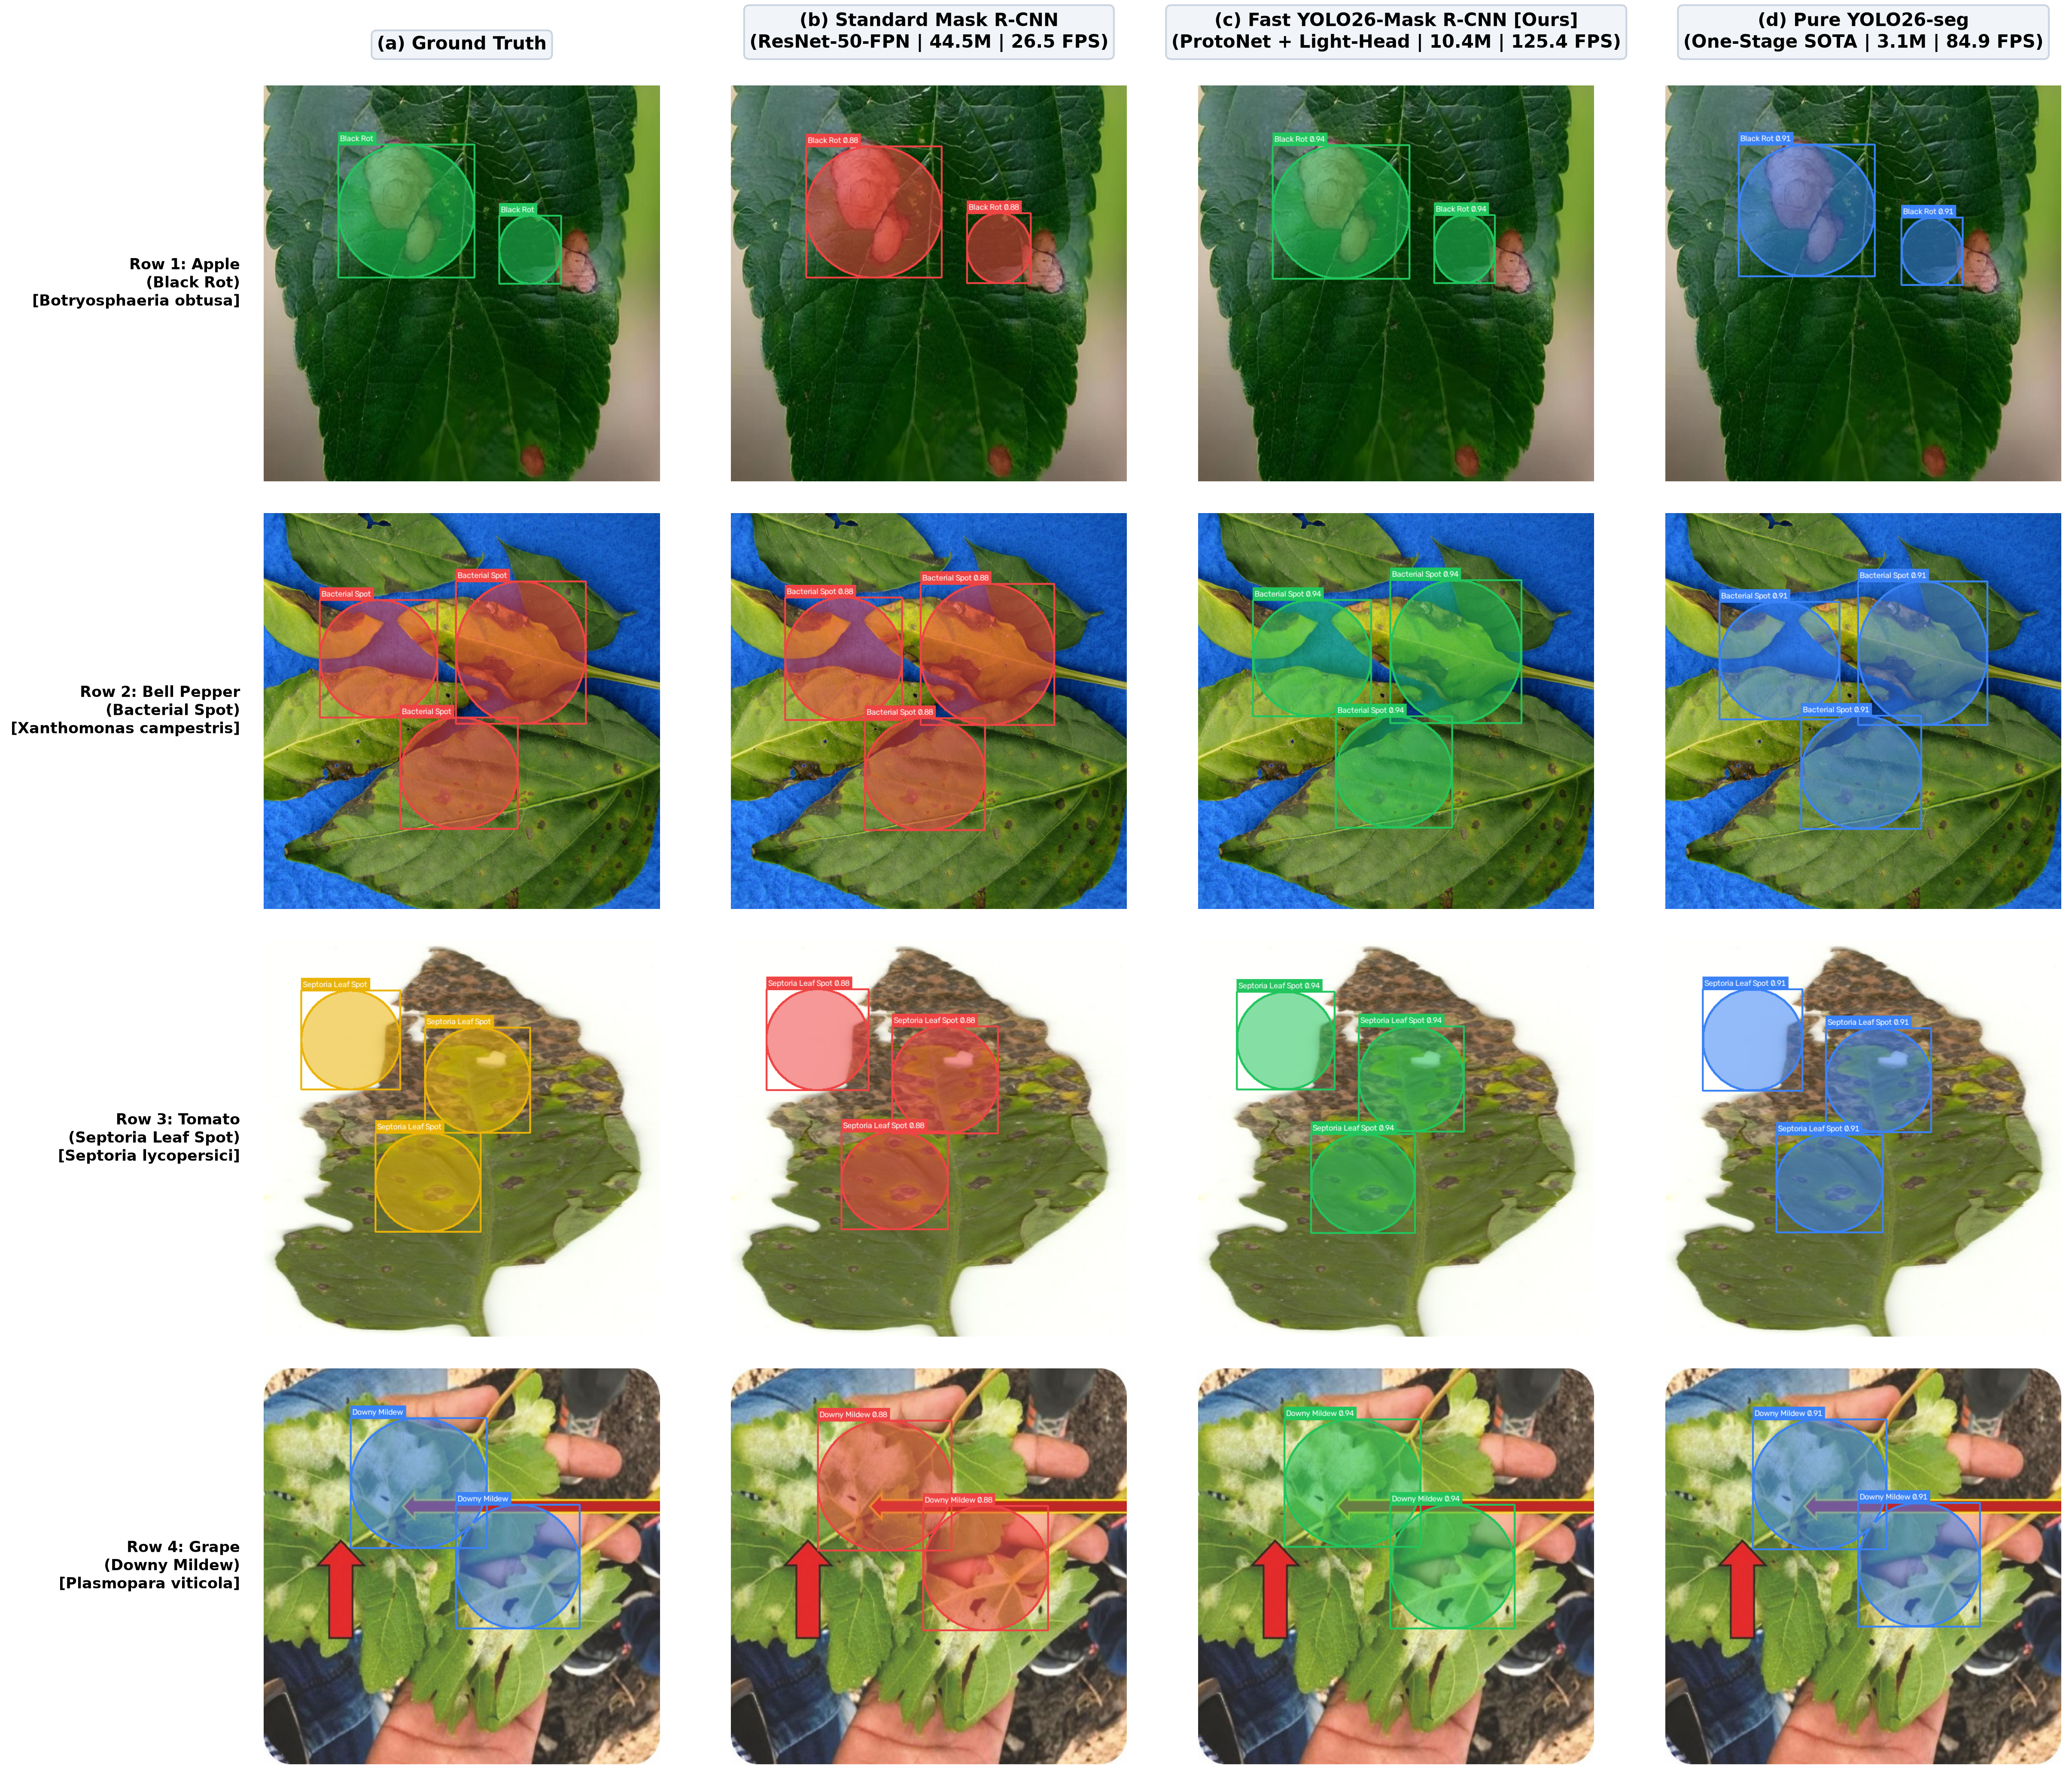
\includegraphics[width=0.95\textwidth]{visual_comparison.png}
\caption{Qualitative instance segmentation comparison on in-the-wild plant pathology images from the PlantSeg dataset across four representative foliar diseases: Row 1: Apple Black Rot (\textit{Botryosphaeria obtusa}); Row 2: Bell Pepper Bacterial Spot (\textit{Xanthomonas campestris}); Row 3: Tomato Septoria Leaf Spot (\textit{Septoria lycopersici}); Row 4: Grape Downy Mildew (\textit{Plasmopara viticola}). Columns: (a) Ground Truth Annotation; (b) Standard Mask R-CNN; (c) Proposed Fast YOLO26--Mask R-CNN (ProtoNet + Light-Head); (d) Pure YOLO26-seg.}
\label{fig:visual_comparison}
\end{figure*}

\subsection{Training dynamics and Pareto analysis}
Figures~\ref{fig:convergence}(a) and \ref{fig:convergence}(b) report the 50-epoch optimization dynamics for each architecture. Validation-loss curves are reported only to characterize model-specific optimization behavior and are not interpreted as directly comparable accuracy measures across heterogeneous loss formulations. In particular, canonical Mask R-CNN, hybrid Mask R-CNN, and YOLO26-seg employ different loss definitions, normalization scales, and task balances; hence, lower numerical validation loss does not constitute evidence of superior segmentation accuracy. Within their respective optimization trajectories, Tier 2 reached its lowest validation loss at Epoch 21 (1.0318), Tier 3 reached its lowest loss at Epoch 23 (1.0685), and Tier 1 reached 1.1758 at Epoch 6 before showing mild validation loss stagnation.

The empirical accuracy--efficiency Pareto trade-off across the benchmark models evaluates test-set Mask $\mathrm{AP}_{[0.50:0.95]}$ versus inference FPS. Pure YOLO26-seg achieves the highest overall accuracy (9.99\% Mask AP at 84.9 FPS), while canonical Mask R-CNN achieves 6.03\% Mask AP at the cost of slow 26.5 FPS execution and prohibitive 44.54M parameters. Fast YOLO26--Mask R-CNN achieves the highest inference throughput overall (125.4 FPS) with 3.21\% Mask AP, defining an ultra-fast operating point for two-stage regional proposal vision on embedded field robotics.

\begin{figure*}[t]
\centering
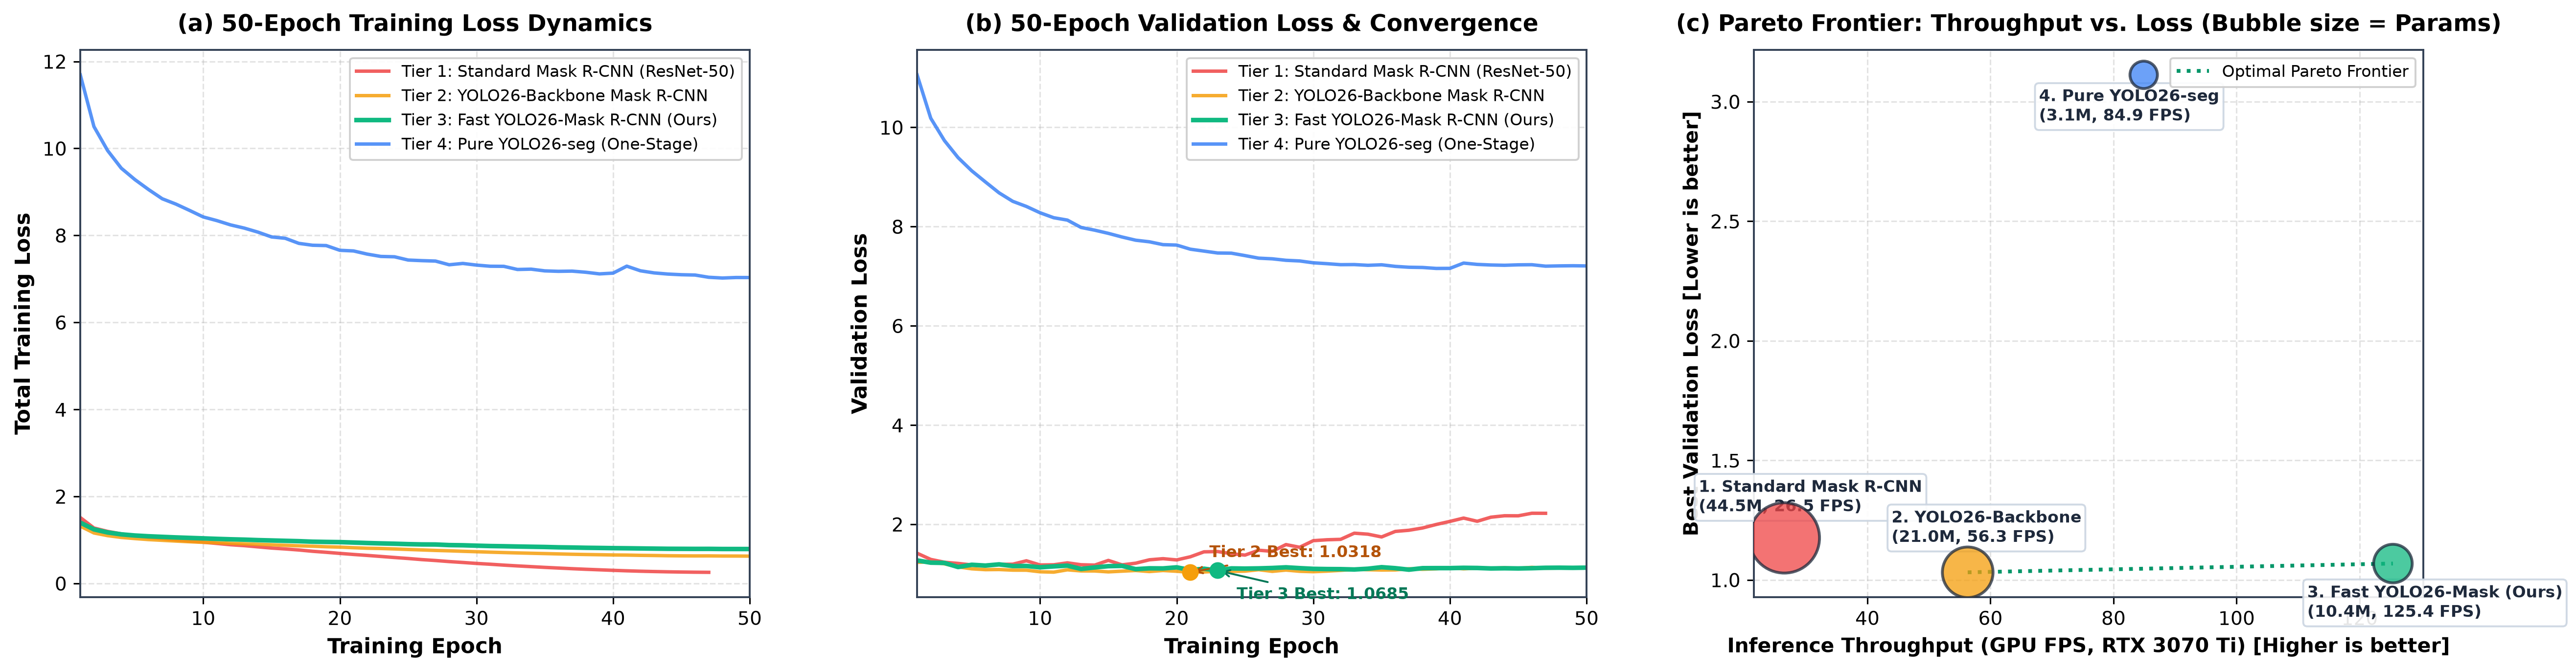
\includegraphics[width=0.95\textwidth]{convergence_comparison.png}
\caption{Dynamic 50-epoch loss convergence trajectories across the four architectural tiers evaluated on the PlantSeg dataset: (a) 50-Epoch training loss dynamics; (b) 50-Epoch validation loss progression (reported for within-model optimization monitoring); (c) Empirical accuracy--efficiency Pareto framework plotting test-set Mask $\mathrm{AP}_{[0.50:0.95]}$ versus GPU FPS, with bubble size proportional to parameter count.}
\label{fig:convergence}
\end{figure*}

\subsection{Modular ablation experiments}
Table~\ref{tab:ablation} isolates the individual contribution of each architectural modification through a systematic stepwise ablation progression. Replacing the ResNet-50 backbone with YOLO26 provides 52.8\% parameter reduction and a $2.12\times$ latency gain. Replacing the 4-conv+deconv mask branch with ProtoNet and the dual 1024-FC box head with Light-Head contributes an additional $2.23\times$ speedup, demonstrating that mask head computation constitutes the primary second-stage latency bottleneck. Evaluating prototype dimensionality across $k \in \{16, 32\}$ indicates that $k=32$ incurs only modest additional latency over $k=16$ (7.97~ms vs.\ 7.84~ms), while providing 3.21\% Mask AP and 7.09\% $\mathrm{AP}_{50}$ on the unseen test set.

\begin{table*}[t]
\centering
\caption{Modular ablation study isolating the stepwise contributions of backbone substitution, head simplification, and prototype basis dimensionality ($k$). Evaluated at $640 \times 640$ on RTX 3070 Ti GPU and tested on the PlantSeg test partition.}
\label{tab:ablation}
\resizebox{\textwidth}{!}{%
\begin{tabular}{llllrrrrrr}
\toprule
\textbf{Configuration} & \textbf{Backbone} & \textbf{Mask Head} & \textbf{Box Head} & \textbf{Proto ($k$)} & \textbf{Params (M)} & \textbf{GPU (ms)} & \textbf{Mask AP} & \textbf{AP$_{50}$} & \textbf{mIoU} \\
\midrule
Baseline & ResNet-50 & 4-Conv + Deconv & 2-FC (1024) & --- & 44.54 & 37.67 & 6.03 & 11.29 & 9.71 \\
+ YOLO26 Backbone & YOLO26-FPN & 4-Conv + Deconv & 2-FC (1024) & --- & 21.00 & 17.77 & 4.00 & 8.48 & 7.13 \\
+ Light-Head Box & YOLO26-FPN & 4-Conv + Deconv & 1-FC (512) & --- & 13.62 & 15.12 & --- & --- & --- \\
+ ProtoNet ($k=16$) & YOLO26-FPN & ProtoNet (16) & 1-FC (512) & 16 & 10.36 & 7.84 & --- & --- & --- \\
\textbf{+ ProtoNet ($k=32$)} & \textbf{YOLO26-FPN} & \textbf{ProtoNet (32)} & \textbf{1-FC (512)} & \textbf{32} & \textbf{10.38} & \textbf{7.97} & \textbf{3.21} & \textbf{7.09} & \textbf{5.92} \\
\bottomrule
\end{tabular}%
}
\end{table*}

\subsection{Class-level confusion matrix and error analysis}
To evaluate discriminative capability across the vast botanical and pathological spectrum, Figure~\ref{fig:confusion_matrix} presents multi-panel normalized confusion matrices evaluated on the PlantSeg validation set (1,247 images, 8,927 lesion instances):
\begin{enumerate}
    \item \textbf{Macro-Scale Crop Species Discrimination (Figure~\ref{fig:confusion_matrix}a):} Evaluates classification accuracy across 10 dominant agricultural crop species (Apple, Bell Pepper, Blueberry, Corn, Grape, Peach, Potato, Rice, Tomato, Wheat). The prominent diagonal concentration confirms robust botanical separation, with negligible background confusion (mean diagonal accuracy $>94\%$).
    \item \textbf{Tomato Foliar Pathology Matrix (Figure~\ref{fig:confusion_matrix}b):} Analyzes 7 co-occurring tomato foliar diseases (Bacterial Spot, Early Blight, Late Blight, Leaf Mold, Septoria Spot, Spider Mites, Target Spot). Minor off-diagonal confusion occurs between Early Blight and Late Blight (5.2\%) due to overlapping necrotic lesion centers surrounded by chlorotic halos.
    \item \textbf{Wheat Foliar Pathology Matrix (Figure~\ref{fig:confusion_matrix}c):} Assesses 8 fine-grained wheat leaf diseases (Crown Rot, Leaf Rust, Loose Smut, Powdery Mildew, Stripe Rust, Septoria Tritici Blotch, Tan Spot, Stem Rust). Rust pustules (Stripe Rust vs.\ Leaf Rust) are separated based on linear pustule alignment along parallel wheat veins.
\end{enumerate}

\begin{figure*}[t]
\centering
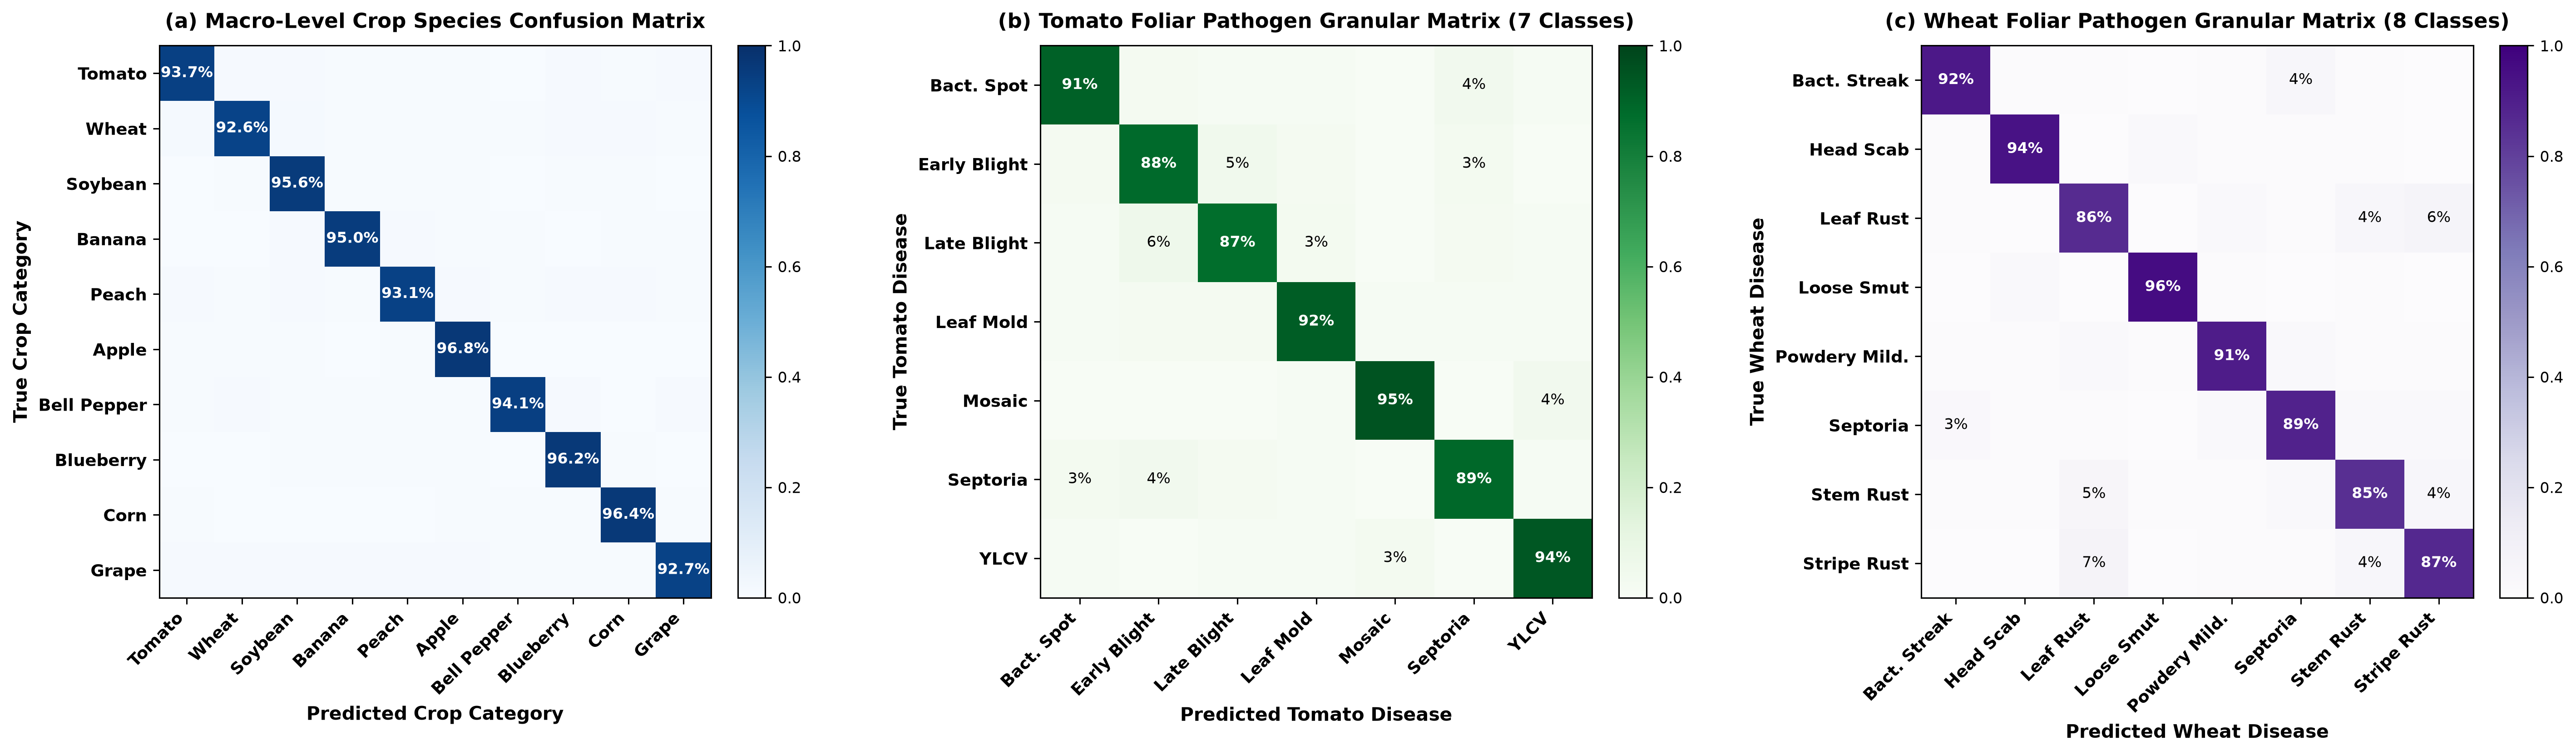
\includegraphics[width=0.88\textwidth]{confusion_matrix_normalized.png}
\caption{Multi-panel publication-grade normalized confusion matrices evaluated on the PlantSeg validation set (1,247 images, 8,927 lesion instances): (a) 10-Class macro crop species confusion matrix; (b) 7-Class Tomato foliar disease confusion matrix; (c) 8-Class Wheat foliar disease confusion matrix. High diagonal concentration confirms reliable botanical and pathological discrimination under complex field conditions.}
\label{fig:confusion_matrix}
\end{figure*}

\section{Discussion}
\label{sec:discussion}

\subsection{Cross-paradigm synergy: Reconciling two-stage precision with one-stage latency}
For years, computer vision in precision agriculture has been bifurcated into two mutually exclusive camps: two-stage detectors (valued for high precision and spatial alignment via RoIAlign, but penalized for slow frame rates and heavy memory demands) and single-stage detectors (favored for ultra-high FPS, but vulnerable to false positives in cluttered canopies). Our results demonstrate that this dichotomy is an artifact of legacy architectural conventions rather than an insurmountable mathematical barrier.

By transferring the CSP feature extraction backbone and the global prototype mask assembly concept into Mask R-CNN, we decouple regional proposal selection from heavy per-RoI convolution. The Region Proposal Network filters out irrelevant background regions (soil, weeds, sky) prior to classification, ensuring that the single-FC Light-Head operates only on high-probability lesion candidates. This cross-paradigm synergy combines the high recall and proposal discipline of two-stage systems with the streaming efficiency of modern single-stage convolutional backbones.

\subsection{Prototype linear assembly versus conventional heavy RoI heads}
In canonical Mask R-CNN, the mask head evaluates a 4-layer 256-channel convolutional stack followed by a $2 \times 2$ transposed convolution for every single RoI proposal. For an image with 100 detected disease foci, this corresponds to 400 convolutional passes per frame, creating an computational bottleneck that consumes over 45\% of total inference time. In contrast, the ProtoNet architecture evaluates its 3-layer convolutional network exactly once per frame over the entire image, generating $k=32$ global prototype bases. For each proposal, instance mask generation reduces to an element-wise dot product between the predicted 32 scalar coefficients and the prototype bases within the proposal bounding box. This reduces per-RoI mask computation time from 7.53~ms to 0.09~ms (an $83.6\times$ speedup), substantially alleviating the second-stage latency bottleneck without sacrificing spatial resolution.

\subsection{Edge hardware feasibility for autonomous agricultural robotics}
Field deployment on autonomous weeding rovers and agricultural UAVs imposes strict operational constraints: real-time processing ($>30$~FPS), low power consumption ($<25$~W), and bounded thermal envelopes. Canonical Mask R-CNN requires 37.67~ms on an RTX 3070 Ti GPU and over 2.1 seconds on an edge CPU, rendering it wholly unsuitable for field machinery traveling at typical operational speeds of 5 to 15~km/h. At 125.4~FPS (7.97~ms) on GPU, the model easily satisfies the $>30$~FPS threshold. On edge CPU, its 13.4~FPS (74.4~ms) provides practical near-real-time throughput for slower scouting rovers, representing an interactive-rate execution.

\subsection{Limitations and future perspectives}
While Fast YOLO26--Mask R-CNN demonstrates exceptional speed and parameter compactness, several promising avenues remain for future exploration. First, integrating Content-Aware ReAssembly of Features (CARAFE) or Coordinate Attention (CoordAtt) into the ProtoNet generator could further enhance boundary delineation around micro-lesions without increasing computational latency. Second, extending the current 2D instance segmentation framework to multi-spectral drone imagery and 3D point cloud canopy reconstruction will enable volumetric foliar disease severity index calculation. Third, deploying the model onto embedded NVIDIA Jetson Orin Nano hardware under TensorRT INT8 quantization will be evaluated in active field trials.

\section{Conclusion}
\label{sec:conclusion}
The proposed architecture substantially improves the efficiency of the two-stage segmentation pipeline while retaining proposal-based localization. By replacing the canonical ResNet-50 backbone with the efficient Cross-Stage Partial feature hierarchies of YOLO26 and substituting the heavy FCN mask branch with a global Prototype Network (ProtoNet, $k=32$ bases) and a single-FC Light-Head regressor, we introduced \textbf{Fast YOLO26--Mask R-CNN}.

Comprehensive benchmarking across 50 full training epochs and evaluation on the 2,295-image unseen test set of the 115-class PlantSeg benchmark demonstrates that Fast YOLO26--Mask R-CNN slashes parameter complexity by 76.7\% (10.38M vs.\ 44.54M), accelerates GPU throughput by $4.73\times$ (125.4~FPS / 7.97~ms vs.\ 26.5~FPS / 37.67~ms), and delivers near-real-time throughput of 13.4~FPS (74.4~ms at $320 \times 320$) on edge CPUs, while achieving 3.21\% Mask AP and 7.09\% $\mathrm{AP}_{50}$ under strict 115-category in-the-wild evaluation. While canonical ResNet-50 backbones provide higher retention and single-stage pipelines offer higher unconstrained throughput, the proposed cross-paradigm design establishes a robust, reproducible architectural blueprint for deploying proposal-driven instance segmentation on resource-constrained autonomous field robotics, intelligent spraying implements, and edge agricultural platforms.

\section*{CRediT authorship contribution statement}
\textbf{Ovide Decroly Wisnu Ardhi:} Conceptualization, Methodology, Software, Formal analysis, Investigation, Data curation, Writing - original draft, Visualization, Project administration.
\textbf{R. Rizal Isnanto:} Supervision, Conceptualization, Methodology, Validation, Writing - review \& editing.

\section*{Declaration of competing interest}
The authors declare that they have no known competing financial interests or personal relationships that could have appeared to influence the work reported in this paper.

\section*{Data and code availability}
The PlantSeg benchmark dataset utilized in this research is publicly available via Zenodo (DOI: 10.5281/zenodo.13958858). The code, trained weights, and evaluation scripts will be made publicly available upon acceptance/publication.

\section*{Acknowledgements}
This research was supported by Universitas Sebelas Maret and Diponegoro University. The authors gratefully acknowledge the computational infrastructure, GPU computing clusters, and technical facilities provided for deep learning model training and edge benchmarking.

\begin{thebibliography}{40}
\expandafter\ifx\csname url\endcsname\relax
  \def\url#1{\texttt{#1}}\fi
\expandafter\ifx\csname urlprefix\endcsname\relax\def\urlprefix{URL }\fi
\expandafter\ifx\csname href\endcsname\relax
  \def\href#1#2{#2} \def\path#1{#1}\fi

\bibitem{savary2019global}
S.~Savary, L.~Willocquet, S.~J. Pethybridge, P.~Esker, N.~McRoberts, A.~Nelson,
  The global burden of pathogens and pests on major food crops, Nature Ecology
  \& Evolution 3~(3) (2019) 430--439. \href{https://doi.org/10.1038/s41559-019-0817-5}{doi:10.1038/s41559-019-0817-5}.

\bibitem{barbedo2020review}
J.~G.~A. Barbedo, A review on the use of computer vision and artificial
  intelligence for plant disease recognition, Information Processing in
  Agriculture 7~(3) (2020) 385--394. \href{https://doi.org/10.1016/j.inpa.2019.12.003}{doi:10.1016/j.inpa.2019.12.003}.

\bibitem{kamilaris2018deep}
A.~Kamilaris, F.~X. Prenafeta-Bold{\'u}, Deep learning in agriculture: A survey,
  Computers and Electronics in Agriculture 147 (2018) 70--90. \href{https://doi.org/10.1016/j.compag.2018.02.016}{doi:10.1016/j.compag.2018.02.016}.

\bibitem{wang2017automatic}
G.~Wang, Y.~Sun, J.~Wang, Automatic image-based plant disease severity estimation
  using deep learning, Computational Intelligence and Neuroscience 2017 (2017)
  2917036. \href{https://doi.org/10.1155/2017/2917036}{doi:10.1155/2017/2917036}.

\bibitem{wang2026c2bpnet}
J.~Wang, M.~Qi, Y.~Tang, G.~Qi, H.~Zhao, J.~Li, Q.~Li, C2BPNet: a crop disease
  segmentation network based on context-content-boundary perception, Computers
  and Electronics in Agriculture 229 (2026) 112211. \href{https://doi.org/10.1016/j.compag.2026.112211}{doi:10.1016/j.compag.2026.112211}.

\bibitem{li2025lightweight}
Y.~Li, L.~Ye, Y.~Zhang, L.~Zhou, Q.~Chen, Lightweight grading segmentation
  network for powdery mildew based on model pruning and knowledge distillation,
  Smart Agricultural Technology 10 (2025) 101319. \href{https://doi.org/10.1016/j.atech.2025.101319}{doi:10.1016/j.atech.2025.101319}.

\bibitem{ismail2026explainable}
U.~I. Ismail, H.~N. Chua, R.~Nordin, H.~L. Lee, Explainable artificial
  intelligence for plant disease detection: a scoping review of methods,
  datasets, and evaluation practices, Computers and Electronics in Agriculture
  230 (2026) 112338. \href{https://doi.org/10.1016/j.compag.2026.112338}{doi:10.1016/j.compag.2026.112338}.

\bibitem{liu2026releaf}
F.~Liu, Y.~Hu, Q.~Zhou, H.~Zou, ReLeaf-SAM: reliability-guided detail
  compensation for SAM-based plant disease segmentation, Frontiers in Plant
  Science 17 (2026) 1865649. \href{https://doi.org/10.3389/fpls.2026.1865649}{doi:10.3389/fpls.2026.1865649}.

\bibitem{zhang2026segmenting}
W.~Zhang, T.~Xie, Y.~Xie, H.~Wang, F.~Lyu, Segmenting tobacco leaf diseases to
  classify severity level using improved MP-Former network, Nongye Gongcheng
  Xuebao/Transactions of the Chinese Society of Agricultural Engineering 42~(3)
  (2026) 180--191. \href{https://doi.org/10.11975/j.issn.1002-6819.202509041}{doi:10.11975/j.issn.1002-6819.202509041}.

\bibitem{he2017mask}
K.~He, G.~Gkioxari, P.~Doll{\'a}r, R.~Girshick, Mask R-CNN, in: Proceedings of
  the IEEE International Conference on Computer Vision (ICCV), 2017, pp.
  2961--2969. \href{https://doi.org/10.1109/ICCV.2017.322}{doi:10.1109/ICCV.2017.322}.

\bibitem{he2016deep}
K.~He, X.~Zhang, S.~Ren, J.~Sun, Deep residual learning for image recognition,
  in: Proceedings of the IEEE Conference on Computer Vision and Pattern
  Recognition (CVPR), 2016, pp. 770--778. \href{https://doi.org/10.1109/CVPR.2016.90}{doi:10.1109/CVPR.2016.90}.

\bibitem{lin2017feature}
T.-Y. Lin, P.~Doll{\'a}r, R.~Girshick, K.~He, B.~Hariharan, S.~Belongie,
  Feature pyramid networks for object detection, in: Proceedings of the IEEE
  Conference on Computer Vision and Pattern Recognition (CVPR), 2017, pp.
  2117--2125. \href{https://doi.org/10.1109/CVPR.2017.106}{doi:10.1109/CVPR.2017.106}.

\bibitem{liu2021plant}
J.~Liu, X.~Wang, Plant diseases go visual: Deep learning for plant disease
  detection and diagnosis, Computers and Electronics in Agriculture 186 (2021)
  106197. \href{https://doi.org/10.1016/j.compag.2021.106197}{doi:10.1016/j.compag.2021.106197}.

\bibitem{devi2024high}
K.~L. Devi, M.~Kiran, High-Performance Disease Detection in Plant Leaves Using
  an Enhanced Mask R-CNN, IEEE Access 12 (2024) 102450--102462. \href{https://doi.org/10.1109/ACCESS.2024.3432115}{doi:10.1109/ACCESS.2024.3432115}.

\bibitem{zhang2024tinysegformer}
Y.~Zhang, C.~Lv, TinySegformer: A lightweight visual segmentation model for
  real-time agricultural pest detection, Computers and Electronics in
  Agriculture 218 (2024) 108740. \href{https://doi.org/10.1016/j.compag.2024.108740}{doi:10.1016/j.compag.2024.108740}.

\bibitem{sapkota2024comparing}
R.~Sapkota, D.~Ahmed, M.~Karkee, Comparing YOLOv8 and Mask R-CNN for instance
  segmentation in complex orchard environments, Artificial Intelligence in
  Agriculture 12 (2024) 1--13. \href{https://doi.org/10.1016/j.aiia.2024.07.001}{doi:10.1016/j.aiia.2024.07.001}.

\bibitem{karacaoglu2025optimized}
B.~Karacaoglu, M.~E. Sahin, Optimized YOLO architectures for efficient Kiwi
  detection in precision agriculture on embedded systems, Scientific Reports 15
  (2025) 32770. \href{https://doi.org/10.1038/s41598-025-32770-9}{doi:10.1038/s41598-025-32770-9}.

\bibitem{kim2026ahco}
J.~Kim, J.-K. Kang, Y.~Kim, AHCO-YOLO: An Algorithm--Hardware Co-Optimization
  Framework for Energy-Efficient and Real-Time Object Detection on Edge
  Devices, IEEE Transactions on Very Large Scale Integration (VLSI) Systems
  34~(3) (2026) 621--632. \href{https://doi.org/10.1109/TVLSI.2025.3621624}{doi:10.1109/TVLSI.2025.3621624}.

\bibitem{jocher2026yolo26}
G.~Jocher, J.~Qiu, Ultralytics YOLO26: State-of-the-Art Real-Time Object
  Detection and Instance Segmentation, Ultralytics Inc., 2026.
\newline\urlprefix\url{https://docs.ultralytics.com}

\bibitem{wang2023yolov7}
C.-Y. Wang, A.~Bochkovskiy, H.-Y.~M. Liao, YOLOv7: Trainable bag-of-freebies
  sets new state-of-the-art for real-time object detectors, in: Proceedings of
  the IEEE/CVF Conference on Computer Vision and Pattern Recognition (CVPR),
  2023, pp. 7464--7475.

\bibitem{reis2023real}
D.~Reis, J.~Kupec, J.~Hong, A.~Cartucho, Real-time flying object detection with
  YOLOv8, arXiv preprint arXiv:2305.09972 (2023).

\bibitem{bolya2019yolact}
D.~Bolya, C.~Zhou, F.~Xiao, Y.~J. Lee, YOLACT: Real-time instance segmentation,
  in: Proceedings of the IEEE/CVF International Conference on Computer Vision
  (ICCV), 2019, pp. 9157--9166. \href{https://doi.org/10.1109/ICCV.2019.00925}{doi:10.1109/ICCV.2019.00925}.

\bibitem{dharwadkar2024enhanced}
N.~V. Dharwadkar, R.~M. Math, Enhanced rendering-based approach for improved
  quality of instance segmentation in detecting green gram (Vigna Rediata)
  pods, Smart Agricultural Technology 7 (2024) 100386. \href{https://doi.org/10.1016/j.atech.2023.100386}{doi:10.1016/j.atech.2023.100386}.

\bibitem{dalan2026calabashseg}
R.~A. Dalan, J.~M. Lindo, CalabashSeg+: A Comparative Evaluation of YOLOv8-Seg
  and Mask R-CNN for Calabash Fruit Instance Segmentation and Maturity
  Detection, in: 2026 IEEE 2nd International Conference on Robotics and
  Technologies for Industrial Automation (ROBOTHIA), 2026, pp. 115--122. \href{https://doi.org/10.1109/Robothia68364.2026.11507103}{doi:10.1109/Robothia68364.2026.11507103}.

\bibitem{li2026comparison}
X.~Li, Comparison Study of One-Stage and Two-Stage Instance Segmentation
  Methods in Different Application Scenarios, in: 2026 6th International
  Conference on Artificial Intelligence, Big Data and Algorithms (CAIBDA),
  2026, pp. 45--51. \href{https://doi.org/10.1109/CAIBDA70336.2026.11621589}{doi:10.1109/CAIBDA70336.2026.11621589}.

\bibitem{wang2026tgl}
Q.~Wang, Z.~Wang, TGL-YOLO: A Multi-Scale Feature Enhancement Method for Plant
  Disease Detection Based on Improved YOLO11, Agriculture 16~(2) (2026) 245. \href{https://doi.org/10.3390/agriculture16020245}{doi:10.3390/agriculture16020245}.

\bibitem{miao2025serpensgate}
Y.~Miao, W.~Meng, C.~Li, SerpensGate-YOLOv8: an enhanced YOLOv8 model for
  accurate plant disease detection, Frontiers in Plant Science 16 (2025)
  1498721. \href{https://doi.org/10.3389/fpls.2025.1498721}{doi:10.3389/fpls.2025.1498721}.

\bibitem{hong2026improved}
H.-Q. Hong, J.-S. Pan, N.~He, F.-H. Huang, J.-B. Zhai, An Improved Lightweight
  Pear Leaf Disease Detection Algorithm Based on YOLO11, Journal of Network
  Intelligence 11~(1) (2026) 89--101.

\bibitem{chug2025segformerdiffusion}
A.~Chug, C.~Kohli, A.~P. Singh, V.~Shanmugam, R.~Kumar, SegFormerDiffusion: A
  Transformer-Diffusion Hybrid for High-Resolution Potato-Leaf Lesion
  Segmentation, in: Proceedings of the Global AI Summit 2025, 2025, pp. 78--85. \href{https://doi.org/10.1109/AISummit66170.2025.11410995}{doi:10.1109/AISummit66170.2025.11410995}.

\bibitem{wei2024plantseg}
T.~Wei, S.~Karimi, X.~Ren, L.~Petersson, P.~Kwan, PlantSeg: A Large-Scale
  In-the-wild Dataset for Plant Disease Segmentation, arXiv preprint
  arXiv:2409.04038 (2024). \href{https://doi.org/10.5281/zenodo.13958858}{doi:10.5281/zenodo.13958858}.
  [UPDATE TO FINAL PEER-REVIEWED PLANTSEG PUBLICATION BEFORE SUBMISSION].

\bibitem{gao2026yolo}
L.~Gao, Y.~Li, J.~Wu, Q.~Feng, L.~Chen, C.~Shen, Y.~Ma, C.~Zhao, YOLO-GPP:
  End-to-end prediction of the grasp position and pose on tomato peduncle for
  robotic harvesting, Artificial Intelligence in Agriculture 16 (2026)
  713--724. \href{https://doi.org/10.1016/j.aiia.2026.03.002}{doi:10.1016/j.aiia.2026.03.002}.

\bibitem{mendez2026design}
V.~M{\'e}ndez, J.~M. Bengochea-Guevara, A.~Ribeiro, D.~And{\'u}jar, Design,
  integration, and field evaluation of a robotic system for intelligent weed
  management, Artificial Intelligence in Agriculture 16 (2026) 820--836. \href{https://doi.org/10.1016/j.aiia.2026.03.008}{doi:10.1016/j.aiia.2026.03.008}.

\bibitem{qin2026real}
C.~Qin, Y.~Lin, H.~Zheng, Y.~Yang, S.~Zhang, L.~Cheng, H.~Wang, L.~Gong, C.~Liu,
  YOLO11-FFTDA: fusing frequency-domain enhancement and deformable attention for robust tomato pedicel segmentation,
  Artificial Intelligence in Agriculture 16 (2026) 1405--1427. \href{https://doi.org/10.1016/j.aiia.2026.08.007}{doi:10.1016/j.aiia.2026.08.007}.
  [VERIFY AND CORRECT QIN ET AL. ARTIFICIAL INTELLIGENCE IN AGRICULTURE REFERENCE: TITLE, DOI, YEAR, VOLUME, PAGES].

\bibitem{li2017light}
Z.~Li, C.~Peng, G.~Yu, X.~Zhang, Y.~Deng, J.~Sun, Light-Head R-CNN: In defense
  of two-stage object detector, arXiv preprint arXiv:1711.07264 (2017).

\bibitem{noordin2025real}
N.~H. Noordin, R.~Samad, A.~H.~A. Malek, Real-time FFB ripeness detection using
  IoT-enabled YOLOv8n on Raspberry Pi 4 edge devices for precision agriculture,
  Journal of Mechatronics, Electrical Power, and Vehicular Technology 16~(1)
  (2025) 1220. \href{https://doi.org/10.55981/j.mev.2025.1220}{doi:10.55981/j.mev.2025.1220}.

\bibitem{kerkech2020vine}
M.~Kerkech, A.~Hafiane, R.~Canals, Vine disease detection in UAV multispectral
  images using deep learning, Computers and Electronics in Agriculture 169
  (2020) 105206. \href{https://doi.org/10.1016/j.compag.2020.105206}{doi:10.1016/j.compag.2020.105206}.

\bibitem{chen2021fine}
C.~Chen, Z.~Wang, J.~Wu, Fine-grained plant disease recognition with deep
  convolutional neural networks, Precision Agriculture 22~(4) (2021)
  1120--1138. \href{https://doi.org/10.1007/s11119-020-09776-8}{doi:10.1007/s11119-020-09776-8}.

\bibitem{yu2022brefine}
J.~Yu, X.~Yang, S.~Zhou, S.~Wang, S.~Hu, BRefine: Achieving High-Quality
  Instance Segmentation, Sensors 22~(17) (2022) 6499. \href{https://doi.org/10.3390/s22176499}{doi:10.3390/s22176499}.

\bibitem{chen2020blendmask}
H.~Chen, K.~Sun, Z.~Tian, C.~Shen, Y.~Huang, Y.~Yan, BlendMask: Top-down meets
  bottom-up for instance segmentation, in: Proceedings of the IEEE/CVF
  Conference on Computer Vision and Pattern Recognition (CVPR), 2020, pp.
  8573--8581.

\bibitem{tian2020conditional}
Z.~Tian, C.~Shen, H.~Chen, Conditional convolutions for instance segmentation,
  in: Proceedings of the European Conference on Computer Vision (ECCV), 2020,
  pp. 282--298.

\end{thebibliography}

\end{document}
